\documentclass[12pt,a4paper]{article}

% --- Encoding & Fonts ---
\usepackage[utf8]{inputenc}
\usepackage[T1]{fontenc}
\usepackage{palatino}
\usepackage{microtype}

% --- Layout ---
\usepackage[top=2.5cm,bottom=2.5cm,left=2.8cm,right=2.8cm,headheight=22pt]{geometry}
\usepackage{parskip}

% --- Colors (from AartShaala logo) ---
\usepackage[dvipsnames]{xcolor}
\definecolor{aartOrange}{HTML}{E8A030}
\definecolor{aartGrey}{HTML}{555555}
\definecolor{aartLightBg}{HTML}{FEF7EC}

% --- Graphics ---
\usepackage{graphicx}
\graphicspath{{./}}

% --- Section headings ---
\usepackage{titlesec}
\titleformat{\section}
  {\color{aartGrey}\large\bfseries}
  {}{0em}{\MakeUppercase}
  [\vspace{2pt}\color{aartOrange}\rule{\linewidth}{1.5pt}\vspace{2pt}]
\titlespacing*{\section}{0pt}{2em}{0.9em}

% --- Lists ---
\usepackage{enumitem}
\setlist[itemize]{
  label={\color{aartOrange}\textbullet},
  leftmargin=1.5em,
  itemsep=0.25em,
  parsep=0pt,
  topsep=0.4em,
}

% --- Wrapping figures ---
\usepackage{wrapfig}

% --- Tier boxes ---
\usepackage[most]{tcolorbox}
\tcbset{
  tierbox/.style={
    colback=aartLightBg,
    colframe=aartOrange,
    colbacktitle=aartOrange,
    coltitle=white,
    fonttitle=\bfseries\small,
    boxrule=1pt,
    arc=5pt,
    top=8pt,bottom=10pt,left=10pt,right=10pt,
    toptitle=5pt,bottomtitle=5pt,
  }
}

% --- Header / footer ---
\usepackage{fancyhdr}
\pagestyle{fancy}
\fancyhf{}
\fancyhead[L]{\small\color{aartGrey}\textit{AartShaala\enspace\textbf{|}\enspace Partnership Proposal}}
\fancyhead[R]{
\includegraphics[height=1.1cm]{logo.png}}
\fancyfoot[C]{\small\color{aartGrey}\thepage}
\renewcommand{\headrulewidth}{0pt}

% --- Rupee sign ---
\newcommand{\rs}{Rs.\,}

% --- Misc ---
\usepackage[hidelinks]{hyperref}
\setlength{\parindent}{0pt}

% ================================================================
\begin{document}

% ================================================================
%  COVER PAGE
% ================================================================
\thispagestyle{empty}

\vspace*{0.5cm}

\begin{flushright}
  
\includegraphics[width=4.2cm]{logo.png}
\end{flushright}

\vspace{2.8cm}

\begin{center}
  {\fontsize{30}{38}\selectfont\color{aartOrange}\textbf{SAMAY KE GHUNGROO}}\\[0.7em]
  {\Large\color{aartGrey}\textit{A Journey Through the Evolution of Kathak}}\\[1.8em]
  {\color{aartOrange!60}\rule{9cm}{0.6pt}}\\[1.8em]
  {\large\color{aartGrey}\textsc{Partnership Proposal}}
\end{center}

\vspace{2cm}

\noindent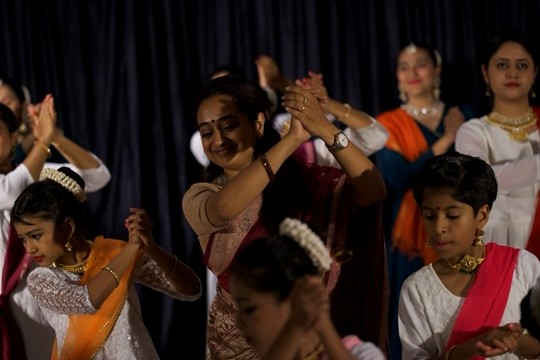
\includegraphics[width=\linewidth]{1.png}

\newpage

% ================================================================
%  ABOUT AARTSHAALA
% ================================================================
\section*{About AartShaala}

AartShaala was established in 2014 with the objective of creating a serious and accessible
learning environment for Kathak and Indian folk dance students. Over the years, the
institution has engaged more than 400 students through regular training, workshops and
performance opportunities across India and internationally. The Bangalore chapter was
established in 2022 and currently trains over 45 students.

The focus at AartShaala is simple: strong fundamentals, disciplined learning and meaningful
performance experiences. Students are encouraged to develop technical proficiency while
building confidence, commitment, a sense of community and an appreciation for the performing
arts.

Today, AartShaala continues to operate as a growing community of students, parents and art
enthusiasts brought together by a shared interest in learning and experiencing Kathak.

% ================================================================
%  ABOUT THE FOUNDER
% ================================================================
\section*{About the Founder}

\begin{wrapfigure}{r}{0.40\textwidth}
  \vspace{-0.5em}
  \centering
  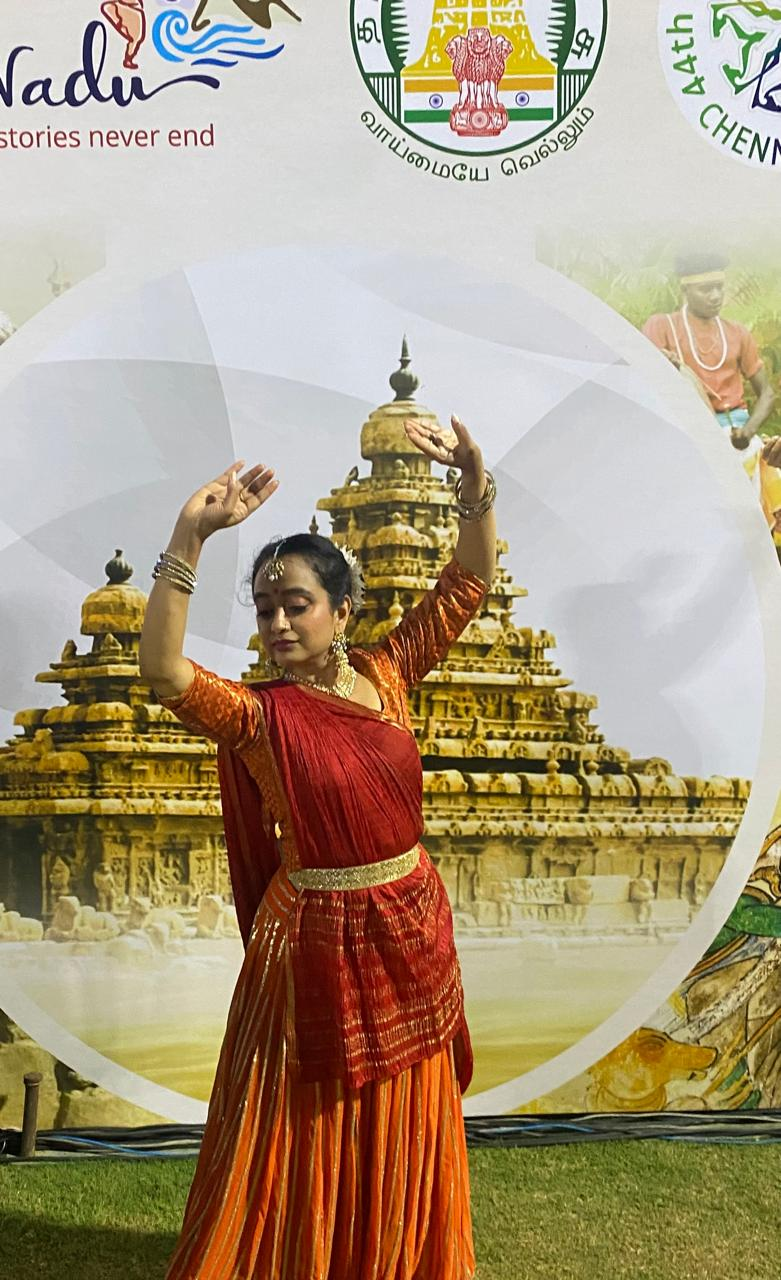
\includegraphics[width=0.38\textwidth,height=9.5cm,keepaspectratio]{2.png}
  \vspace{-1em}
\end{wrapfigure}

Rupini Raman is a senior Human Resources leader, Kathak artist and founder of AartShaala.

A student of Kathak for over three decades, she has pursued her artistic journey alongside
a full-time corporate career, balancing leadership responsibilities with rigorous training,
performance and teaching.

She is a Doordarshan Graded Artist, holds a Bachelor's Degree in Kathak and is currently
pursuing her Master's Degree in the discipline.

Her artistic journey began under the tutelage of the late \textbf{Shri Vishaka Mathur Ji},
whose foundational teachings continue to shape her practice. She currently pursues her
training under the guidance of \textbf{Guru Neha Banerjee} and \textbf{Guru Saswati Sen Ji}.

In 2014, she founded AartShaala with the intention of creating a structured and nurturing
environment for students interested in learning Kathak. Over the last decade, she has
trained and mentored hundreds of students through regular classes, workshops and stage
productions.

Beyond the classroom, Rupini is committed to making arts education accessible to children
who may otherwise never have the opportunity to learn. Through AartShaala, she personally
sponsors the dance education of children from underserved communities, including the
children of domestic workers, drivers and gig workers, covering their tuition, examination
fees, costumes and performance expenses.

She also actively creates opportunities for local folk artists by connecting them with
corporate platforms and cultural events, enabling them to showcase their talent and earn
with dignity. Her belief is simple: art should not be a privilege reserved for a few; it
should be accessible, inclusive and capable of transforming lives.

Her belief is straightforward: while careers and professional identities are important,
every individual benefits from having an artistic pursuit in life. Art develops discipline,
focus, confidence and creativity, and often becomes a lifelong source of joy and personal
fulfilment.

Through AartShaala, she hopes to make that experience available to more students and
families.

\begin{center}
  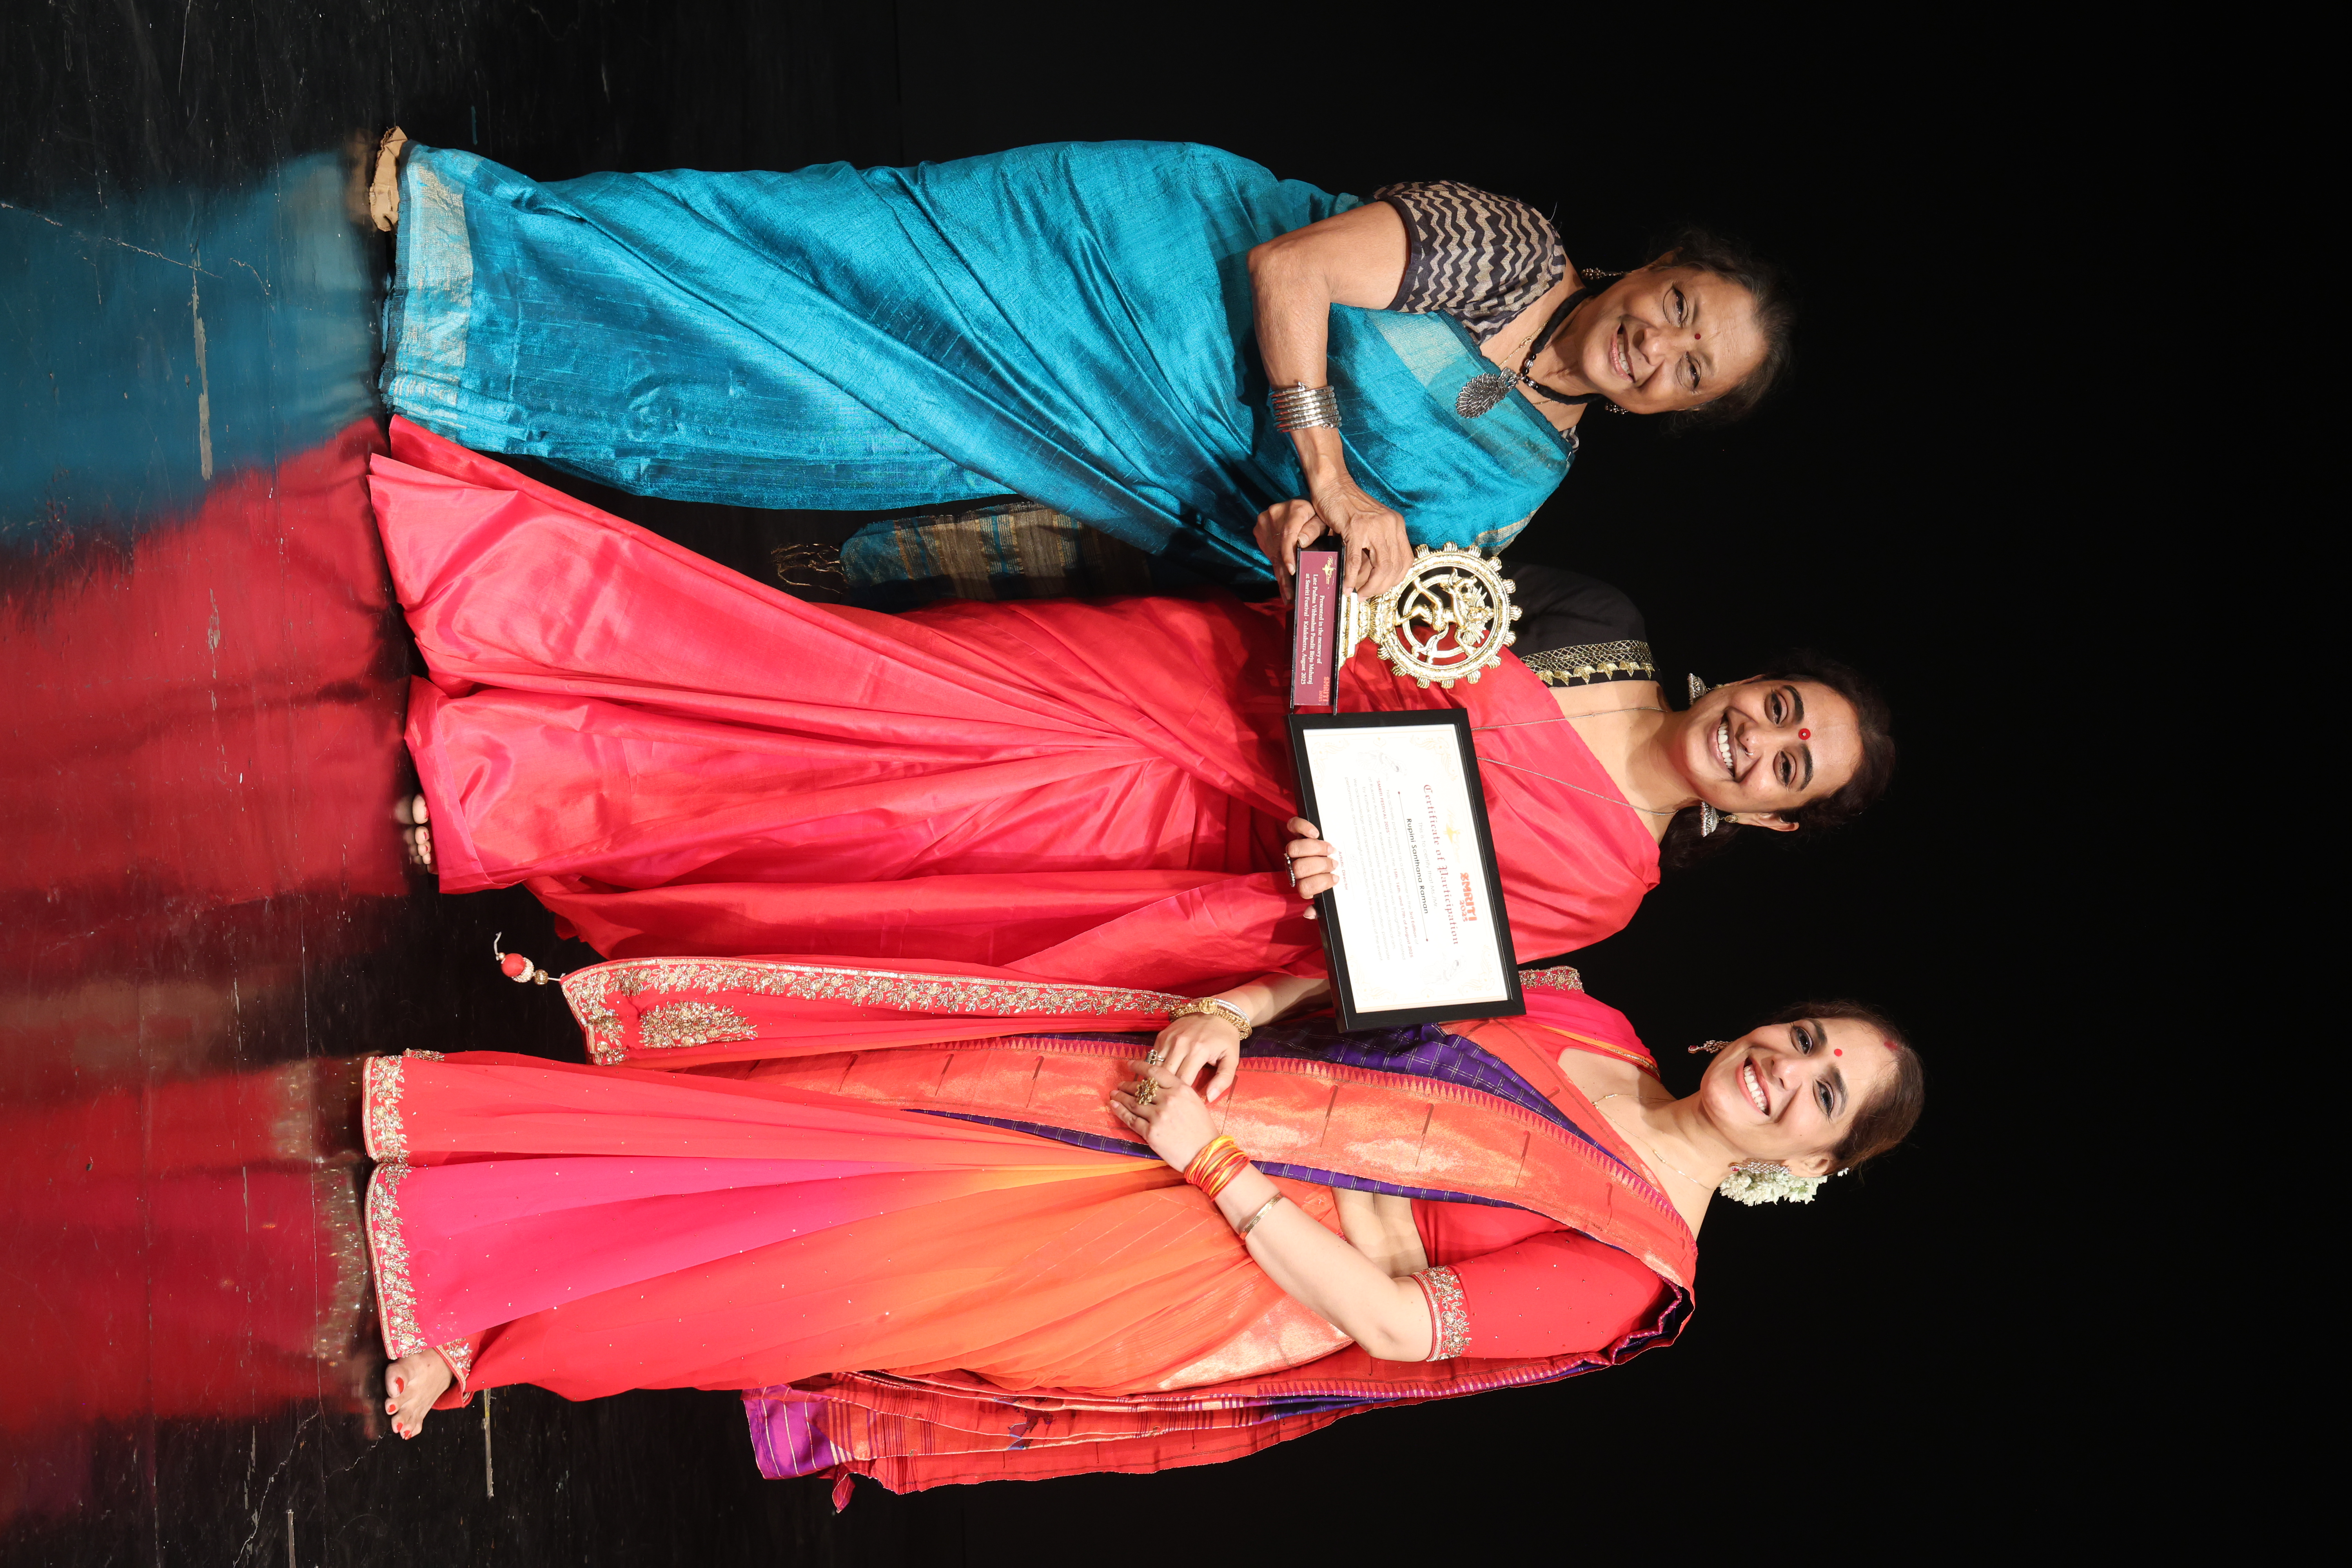
\includegraphics[width=0.82\linewidth,angle=90,origin=c]{rupini_with_gurus.JPG}\\[0.5em]
  \small\color{aartGrey}\textit{(L to R) Guru Saswati Sen Ji\enspace|\enspace Rupini Raman\enspace|\enspace Guru Neha Banerjee}
\end{center}
\newpage
% ================================================================
%  ABOUT THE PRODUCTION
% ================================================================
\section*{About the Production: \textit{Samay Ke Ghungroo}}

\textit{Samay Ke Ghungroo} is AartShaala's annual showcase, the first in Bangalore.
This year's theme explores the evolution of Kathak through time.

Through dance, music and storytelling, students will present Kathak's journey from its
origins as a storytelling tradition to its development through royal courts and its
expression on contemporary stages today.

The production is an opportunity for students to experience the discipline and excitement
of presenting a professional performance while deepening their understanding of the history
and heritage of the art form they learn.

% ================================================================
%  EVENT DETAILS
% ================================================================
\section*{Event Details}

\noindent
\begin{minipage}[t]{0.44\textwidth}
  \textbf{\color{aartOrange}Venue}\\[0.4em]
  Bangalore International Centre (BIC)

  \bigskip
  \textbf{\color{aartOrange}Date}\\[0.4em]
  4 September 2026

  \bigskip
  \textbf{\color{aartOrange}Audience}\\[0.4em]
  Approximately 180 invited guests
\end{minipage}%
\hfill
\begin{minipage}[t]{0.52\textwidth}
  \textbf{\color{aartOrange}The audience will include:}
  \begin{itemize}
    \item Families and parents
    \item Cultural enthusiasts
    \item Professionals and entrepreneurs
    \item Educators and artists
    \item Members of Bangalore's arts community
  \end{itemize}
\end{minipage}

\medskip
The event brings together individuals who value learning, culture, tradition and community.

% ================================================================
%  AARTSHAALA AT A GLANCE
% ================================================================
\section*{AartShaala at a Glance}

\begin{itemize}
  \item 400+ students engaged through regular training and workshops
  \item Students across India and internationally
  \item 2026 Annual showcase hosted at Bangalore International Centre
  \item Founded and led by Rupini Raman, Doordarshan Graded Artist
  \item Dedicated to making Indian classical arts accessible to the next generation
  \item Focused on learning, performance and cultural appreciation through Kathak
\end{itemize}

\newpage

% ================================================================
%  WHY THIS MATTERS
% ================================================================
\section*{Why This Matters}

\noindent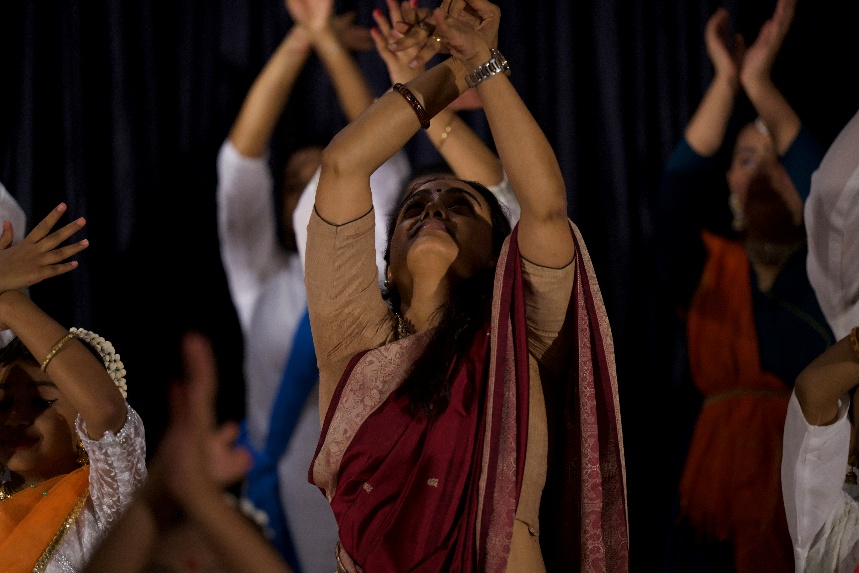
\includegraphics[width=\linewidth]{3.png}

\medskip

In an increasingly fast-paced world, opportunities for young people to engage deeply with
the arts are becoming fewer. Yet art continues to play an important role in shaping
confidence, creativity, discipline and self-expression. It keeps us connected to our roots
while helping us navigate a rapidly changing world.

Not every child who learns an art form will become a professional artist, nor should that
be the goal. However, every child can benefit from the experience of learning, practising
and appreciating an art form.

\textit{Samay Ke Ghungroo} seeks to create that opportunity, allowing students to learn
from tradition, perform with confidence and experience the joy of being part of something
larger than themselves.
\newpage
% ================================================================
%  PARTNERSHIP OPPORTUNITIES
% ================================================================
\section*{Partnership Opportunities}

We invite individuals and organisations who value education, culture and community to
support this initiative.

\bigskip

\noindent
\begin{minipage}[t][17cm][c]{0.54\textwidth}
  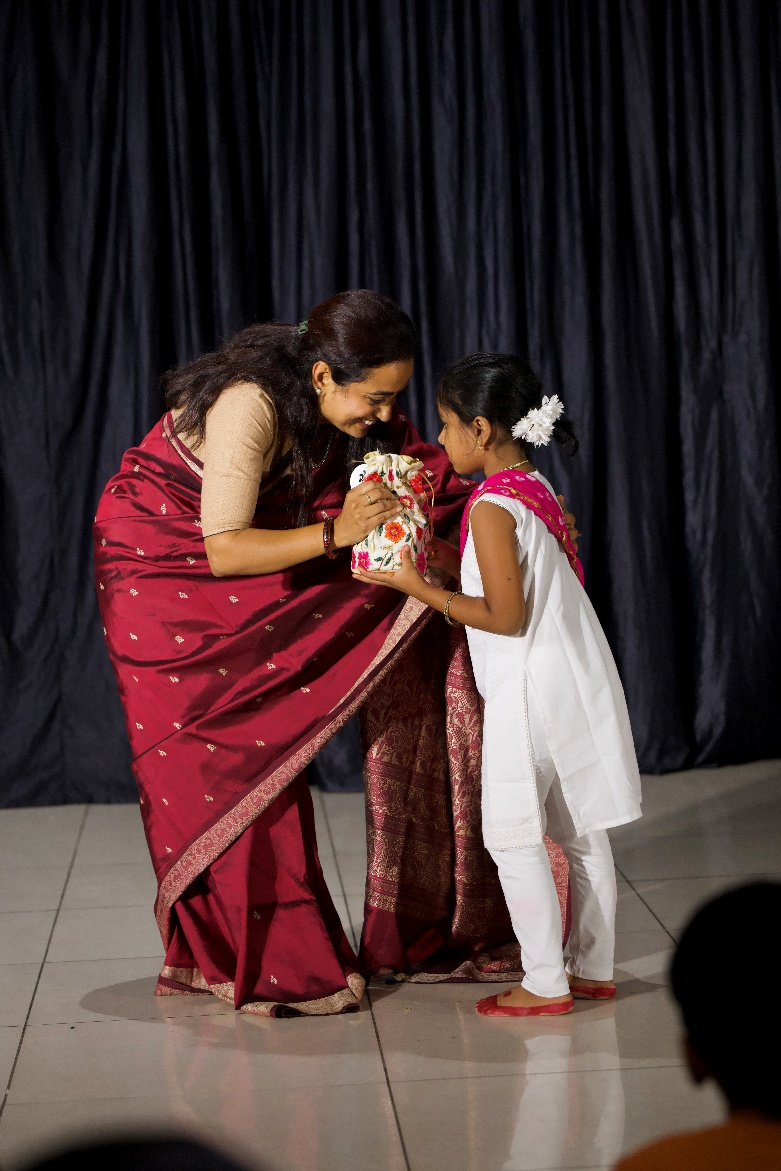
\includegraphics[width=\linewidth]{4.png}
\end{minipage}%
\hfill
\begin{minipage}[t][17cm][s]{0.42\textwidth}
\small
  % --- Tier 1 ---
  \noindent{\color{aartOrange}\rule{\linewidth}{1.5pt}}\\[0.3em]
  {\bfseries\color{aartGrey} Patron Partner\,/\,Platinum Sponsor}
  \hfill{\normalsize\bfseries\color{aartOrange}\rs75,000}\\[0.2em]
  \begin{itemize}[leftmargin=1.2em,itemsep=0.2em,topsep=0.1em]
    \item Principal acknowledgement across all event communications
    \item Premium visibility in event brochure and passes
    \item Acknowledgement during the event
    \item Foyer standee placement
    \item Reserved seating for guests
  \end{itemize}

  \vfill

  % --- Tier 2 ---
  \noindent{\color{aartOrange}\rule{\linewidth}{1.5pt}}\\[0.4em]
  {\bfseries\color{aartGrey} Cultural Partner\,/\,Gold Sponsor}
  \hfill{\normalsize\bfseries\color{aartOrange}\rs40,000}\\[0.2em]
  \begin{itemize}[leftmargin=1.2em,itemsep=0.2em,topsep=0.1em]
    \item Visibility in event brochure
    \item Acknowledgement during the event
    \item Foyer standee placement
    \item Reserved seating
  \end{itemize}

  \vfill

  % --- Tier 3 ---
  \noindent{\color{aartOrange}\rule{\linewidth}{1.5pt}}\\[0.4em]
  {\bfseries\color{aartGrey} Supporting Partner}
  \hfill{\normalsize\bfseries\color{aartOrange}\rs20,000}\\[0.2em]
  \begin{itemize}[leftmargin=1.2em,itemsep=0.2em,topsep=0.1em]
    \item Visibility in event brochure
    \item Acknowledgement during the event
    \item Reserved seating
  \end{itemize}
  \noindent{\color{aartOrange}\rule{\linewidth}{1.5pt}}

\end{minipage}

\newpage

% ================================================================
%  A PERSONAL NOTE
% ================================================================
\section*{A Personal Note}

\noindent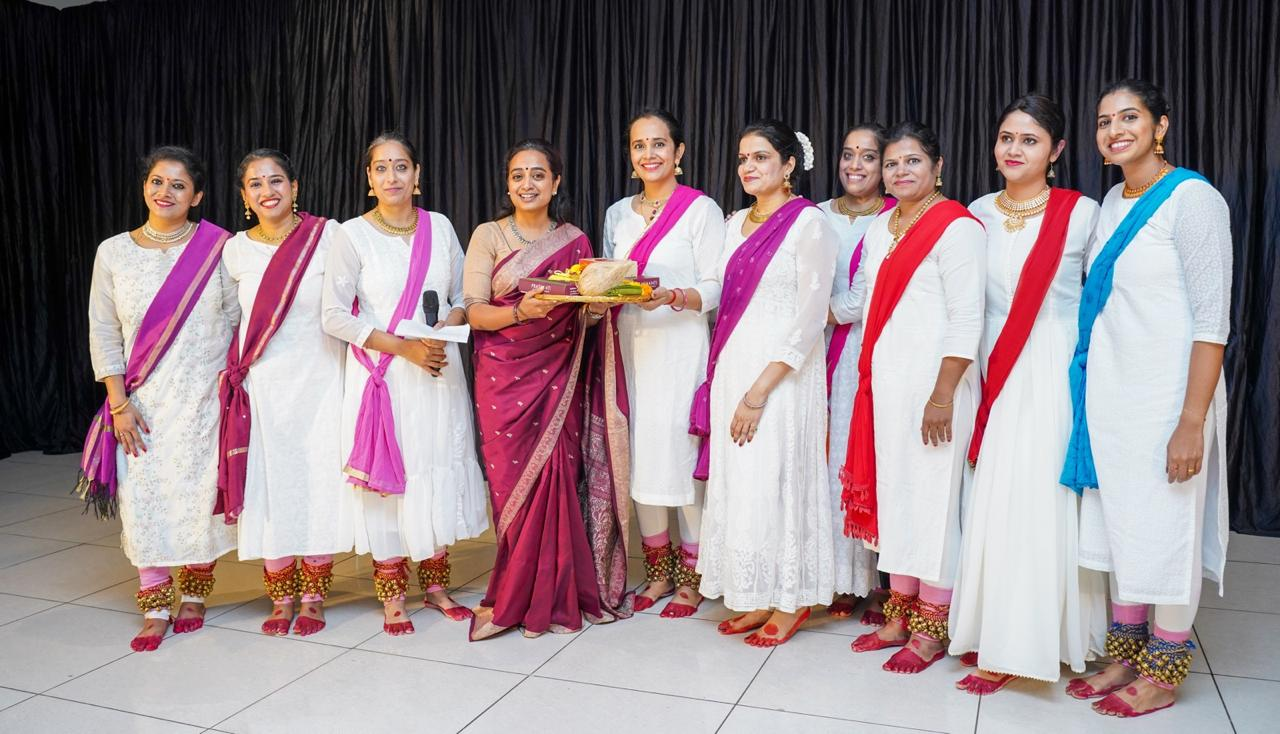
\includegraphics[width=\linewidth]{5.png}

\medskip

AartShaala is a labour of love that has grown steadily over the last decade alongside my
professional career. As someone who has spent many years in corporate leadership while
continuing my own journey as a student and practitioner of Kathak, I have experienced the
value that an artistic pursuit brings to life.

Not every student who learns Kathak will become a performer, and that is perfectly fine.
The objective is not to create professional dancers out of everyone. It is to give young
people an opportunity to learn, commit to something meaningful and experience the
confidence that comes from mastering a craft.

If this vision resonates with you, we would be grateful for your support.

\vspace{1.8em}

With gratitude,

\vspace{0.9em}

\textbf{\color{aartGrey}Rupini Raman}\\[0.3em]
\textit{Founder, AartShaala}\\
\textit{Kathak Artist and Teacher\enspace|\enspace Doordarshan Graded Artist}

\vspace{2.5em}

\noindent{\color{aartOrange}\rule{\linewidth}{1.5pt}}

\vspace{0.8em}

\begin{center}
  \textbf{\color{aartGrey}Get in Touch}\\[0.6em]
  \small
  \textbf{Phone:}\enspace +91\,99622\,27759
  \quad\textbf{|}\quad
  \textbf{Email:}\enspace \href{mailto:rupiniraman@gmail.com}{rupiniraman@gmail.com}\\[0.5em]
  \textbf{Instagram:}\enspace \href{https://www.instagram.com/aartshaala_bangalore/}{@aartshaala\_bangalore}
\end{center}

\end{document}
